\chapter{Porównanie} \label{chap:porownanie}
Choć porównywanie kombinacji bibliotek z językiem programowania wydaje się dziwne, to jeżeli spojrzy się na funkcjonalności oferowane przez Reacta i Reduxa w porównaniu do możliwości Elma, można zauważyć pewne podobieństwa w sposobie budowania aplikacji. W tym rozdziale zostały opisane funkcjonalności, które są oferowane przez oba rozwiązania, oraz różnice występujące między Reactem i~Reduxem a Elmem dla każdej z funkcjonalności.

\section{Virtual DOM i składnia}
% Czym jest DOM?
DOM \footnote{z. ang. Document Object Model} jest niezależnym od platformy i języka programowania interfejsem, który pozwala programom i skryptom na dynamiczny dostęp i aktualizację treści, struktury i stylu dokumentu. Kiedy strona internetowa jest ładowana, przeglądarka tworzy DOM strony, będący obiektową reprezentacją dokumentu HTML. Służy ona jako interfejs umożliwiający pobieranie oraz modyfikację elementów HTML, które w DOM-ie są zdefiniowane jako obiekty.

% Dlaczego DOM jest powolny?
Każda akcja na stronie powoduje zmianę DOM-u. Ze względu na jego drzewiastą strukturę, sama modyfikacja DOM-u jest szybka. Jednak każdy z modyfikowanych elementów oraz wszystkie jego dzieci muszą dodatkowo przejść przez dwa kosztowne etapy:
\begin{enumerate}
	\item Reflow będący procesem, podczas którego przeliczane zostają wymiary oraz pozycja elementu. Dokładnie ten sam proces jest uruchamiany na węzłach dzieci, a także elementach, które pojawiają się w DOM-ie później niż główny element. Reflow jest kosztowny, ponieważ zmiana pojedynczego elementu w strukturze DOM-u może spowodować wywołanie Reflow na wielu innych elementach.
	\item Repaint, w którym niektóre partie ekranu muszą zostać zaktualizowane, czy to ze względu na modyfikacje wymiarów i~pozycji elementu, czy przez zmiany stylistyczne, takie jak zmiana koloru tła. Etap ten jest kosztowny ponieważ przeglądarka musi sprawdzić widoczność innych węzłów w~DOM-ie.
\end{enumerate} 

% Czym jest Virtual DOM?
Virtual DOM jest to lekka, niezależna od przeglądarki abstrakcyjna reprezentacja DOM-u. Służy ona między innymi do zminimalizowania kosztu stworzonego przez etapy Reflow i Repaint. Zamiast tworzyć za każdym razem drzewo składające się z węzłów DOM-u, Virtual DOM pozwala na stworzenie tego drzewa przy pomocy abstrakcyjnych węzłów, które są odpowiednikami faktycznych elementów DOM-u. Dzięki temu wszystkie operacje modyfikujące widok mogą być wykonane na abstrakcyjnej strukturze, a dopiero końcowy rezultat powoduje modyfikację faktycznego DOM-u.

% Diff algorithm
Koncepcja Virtual DOM-u została wykorzystana do tego, aby w każdej klatce budować zupełnie nową scenę. Choć taka operacja wydaje się kosztowna, to tak naprawdę zbudowanie pełnego drzewa Virtual DOM-u jest szybkie, i jest wykorzystywane przy każdej aktualizacji widoku. W momencie gdy następuje zmiana powodująca modyfikację widoku, algorytm porównuje ze sobą stare i nowe drzewo Virtual DOM-u. Wszystkie komponenty, w których nastąpiła jakakolwiek zmiana są oznaczane specjalną flagą, która określa, że dany węzeł został zmodyfikowany. Na tej podstawie budowana jest dokładna lista zmian jakie nastąpiły w widoku. Następnie lista ta jest wykorzystywana do modyfikacji faktycznego DOM-u, lecz nie jako pojedynczo wprowadzane zmiany, a jedna aktualizacja drzewa dokumentu. 

\begin{figure}[h]
	\centering
	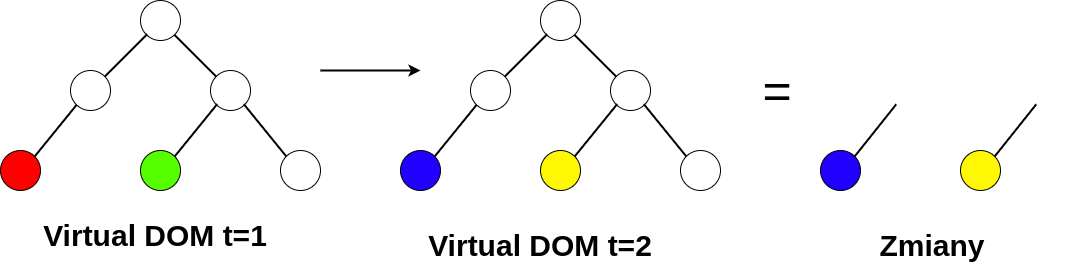
\includegraphics[width=0.8\textwidth]{images/diff_algorithm}
	\caption{Schemat działania algorytmu  porównywania różnic}
	\label{fig:diffAlgorithm}
\end{figure}

%Reprezentacja w React i Elm - składnia
Zarówno React, jak i Elm posiadają własne implementacje Virtual DOM-u. W Elmie abstrakcyjną reprezentację węzła otrzymujemy przy pomocy funkcji \lstinline{node}, która jako atrybuty przyjmuje tag, listą atrybutów HTML, oraz listę węzłów dzieci:
\begin{lstlisting}[style=elm-style]
	node : String -> List Attrbiute -> List Html -> Html
\end{lstlisting}
W przypadku użycia tagów HTML, takich jak \lstinline{div}, Elm udostępnia funkcje pomocnicze, które posiadają już uzupełniony atrybut tag, pozostawiając nam do określenia atrybuty węzła oraz jego dzieci. Elm nie ma specjalnej składni, która służyłaby do budowania widoków. Wszystkie elementy, z których budowany jest widok aplikacji, są funkcjami. W przypadku budowania widoku jedynym wymaganiem jest, aby funkcja go budująca zwracała rekord specjalnego typu \lstinline[style=elm-style]{Html msg}, który jest głównym blokiem służącym do tworzenia wyjściowego kodu HTML.

W przypadku Reacta mamy do czynienia ze znacznie bardziej rozszerzonym podejściem.  Bazowym elementem reprezentującym abstrakcyjny węzeł Virtual DOM-u jest ReactElement. Analogicznie jak w przypadku funkcji \lstinline{node} w Elmie jest to obiekt posiadający informację o tagu, który reprezentuje, atrybutach zdefiniowanego węzła, oraz listę dzieci. Przykład tworzenia takiego elementu można zobaczyć we fragmencie kodu \ref{listing:jsreactelement}. 

\begin{minipage}{.45\textwidth}
	\begin{lstlisting}[caption=Javascript,style=JavaScript,label = listing:jsreactelement]
	var divHello = React.createElement(
	"div",
	{ className: "myclass" },
	"Hello world!"
	);
	\end{lstlisting}
\end{minipage}\hfill
\begin{minipage}{.45\textwidth}
	\begin{lstlisting}[caption=JSX,style=JavaScript,firstnumber=1,label = listing:jsx]
	var divHello = (
	<div className="myclass">
	Hello world!
	</div>
	);
	\end{lstlisting}
\end{minipage}

Biorąc pod uwagę to, że każdy element Virtual DOM-u w React'cie jest zbudowany w podobny sposób, można zauważyć, że w przypadku rozbudowanej aplikacji, kod bardzo szybko staje się skomplikowany i niezrozumiały. Aby tego uniknąć, Facebook stworzył specjalne rozszerzenie składni dla JavaScriptu -- JSX. Z wyglądu przypomina składnię języka HTML, lecz zasadniczo dostarcza cukier syntaktyczny dla funkcji \lstinline[style=JavaScript]{createElement}. Fragmenty kodu \ref{listing:jsx} oraz \ref{listing:jsreactelement} są dokładnie tymi samymi wyrażeniami, z tą różnicą, że w drugim przypadku został wykorzystany JSX. Takie podejście pozwala na użycie JSX-a wewnątrz instrukcji JavaScriptu, przypisywanie go do zmiennych, czy też zwracanie z funkcji. Operacja zachodzi także w drugą stronę, co znaczy, że można korzystać z kodu JavaScriptu wewnątrz składni JSX-a. Taki kod musi być objęty nawiasami klamrowymi, aby odróżnić fragmenty napisane w JavaScript'cie od kodu JSX-a. 

% Test czasu renderowania
Choć główne założenia Virtual DOM-u w Elmie i React'cie są podobne, to jego implementacje nie są identyczne, w związku z czym można je porównać pod względem wydajnościowym. W tym przypadku wykorzystany został test wydajnościowy stworzony przez twórcę Elma \cite{perComp}. Pozwala on na porównanie czasu renderowania różnych implementacji aplikacji TodoMVC. Jest to prosty projekt listy zadań, umożliwiający dodawanie i usuwanie wpisów, oznaczanie ich jako zakończone, a także odfiltrowywanie na podstawie statusu wpisów. Test zakłada realistyczny scenariusz, w którym każda zmiana jest wyświetlona jako pojedyncza klatka, tak jakby to faktyczny użytkownik przeprowadzał test. Algorytm scenariusza wykonywany w trakcie pomiaru średniego czasu renderowania wygląda następująco:
\begin{enumerate}
	\item Stworzenie strony niezawierającej wpisów
	\item Dodanie 100 wpisów do listy
	\item Oznaczenie każdego z elementów jako zakończony
	\item Usunięcie wszystkich wpisów
\end{enumerate}
Dodatkowo zostały przyjęte następujące założenia, które sprawiają, że przeprowadzony test jest sprawiedliwy:
\begin{enumerate}
	\item Brak zgrupowanych zdarzeń -- oznacza to, ze zamiast generować zdarzenia w pojedyńczej pętli, algorytm tworzy jedno zdarzenie na raz, przechodząc do następnego dopiero po wyrenderowaniu całego widoku. Gdyby takie założenie nie zostało przyjęte, to przykładowo w przypadku dodawania wpisów, zmiany następowałyby na tyle szybko, że zamiast wyświetlić 100 klatek, przeglądarka wyświetliłaby tylko jedną.
	\item Brak użycia \lstinline{requestAnimationFrame} -- funkcja ta informuje przeglądarkę o zamiarze wykonania animacji i żąda od przeglądarki wywołania określonej funkcji w celu odświeżenia animacji przed następną zmianą w widoku. Oznacza to, że odświeżenie animacji jest wyrównane do 60 razy na sekundę, niezależnie od tego jak wiele klatek wygeneruje JavaScript. Elm wykorzystuje tą funkcję do pomijania części klatek, które i tak nie będą widoczne dla użytkownika, W z związku z realistycznym scenariuszem, oraz brakiem podobnej optymalizacji w innych implementacjach, funkcja ta musiała zostać usunięta z Elma w ramach przeprowadzanego testu.
\end{enumerate}

\begin{figure}[h]
	\centering
	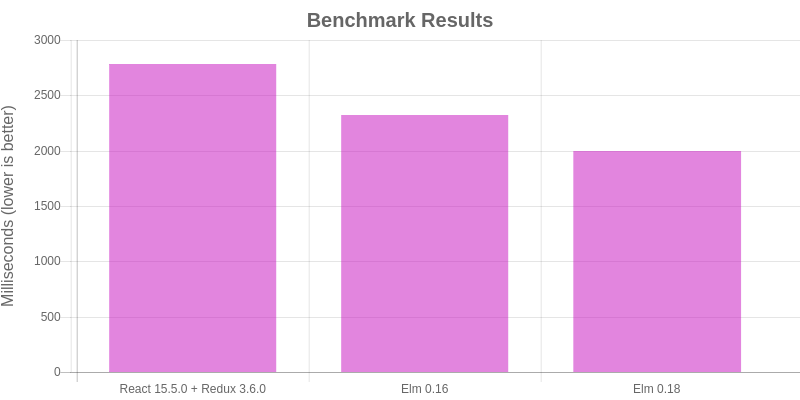
\includegraphics[width=0.9\textwidth]{images/render_comparision}
	\caption{Porównanie czasu renderowania aplikacji TodoMVC (w oparciu o \cite{perComp})}
	\label{fig:performanceComparision}
\end{figure}

Na rysunku \ref{fig:performanceComparision} można zauważyć, że zostały wzięte pod uwagę dwie wersje Elma. Powodem jest tutaj zmiana używanej implementacji Virtual DOM-u. Od początku istnienia Elma aż do wersji 0.16, wykorzystywana była implementacja Matta Escha, która była silnie inspirowana wersją Virtual DOM-u wykorzystywaną w React'cie. Jednak z powodu dużych zmian wprowadzonych w nowszych wersjach Elma, twórca języka był zmuszony stworzyć własną implementację dopasowaną do nowego API. 

Wyniki testu pokazują, że implementacja aplikacji w Elmie jest szybsza o ponad sekundę. Twórca Elma w jednym ze swoich artykułów \cite{blazingFastHtml} pisze o wykorzystanych technikach, które są powodem takich wyników:
\begin{enumerate}
	\item Używanie tablic zamiast słowników -- iteracja po tablicy jest zawsze o wiele szybszaą operacją niż przechodzenie po kluczach słownika
	\item Minimalizacja alokacji -- garbage collection jest jednym z kosztownych elementów w analizowanych implementacjach. Im mniej obiektów jest alokowanych, tym lepsza jest wydajność aplikacji. Sposób wykorzystany w Elmie polega na alokowaniu obiektów z pustymi polami. Dzięki temu silniki JavaScriptowe radzą sobie o wiele lepiej z optymalizacją takich obiektów, a obiekt nie zmienia się, nawet gdy wypełnimy go większą ilością informacji.
	\item Unikanie powolnych operacji, takich jak pobieranie konkretnego elementu z tablicy. 
\end{enumerate}
\section{Jednokierunkowe flow aplikacji}

\section{Niemutowalność obiektów}

\section{Biblioteki i menedżery pakietów}
